In diesem Kapitel soll die Genauigkeit bei der Berechnung von chemischen Abschirmungskonstanten mit unterschiedlichen Funktionaltypen überprüft und die Effizienz der in dieser Arbeit implementierten Verfahren demonstriert werden. Ein besonderes Augenmerk liegt dabei auch auf möglichen Genauigkeitseinbußen aufgrund der verwendeten Näherungsverfahren. Im Detail wurden dafür die $^1$H-, $^{13}$C-, $^{19}$F- und $^{31}$P-chemische Verschiebungen in einem Testsatz von Molekülen untersucht.\supercite{reiter2017calculation} Zur Überprüfung der Genauigkeit der neu implementierten \ac{mgga}-Funktionale wurden zunächst die Berechnungen mit den Funktionalen TPSS\supercite{tao2003climbing} und TPSSh\supercite{staroverov2003comparative} mit den Ergebnissen einer CCSD(T)/cc-pVQZ\supercite{dunning1989gaussian,woon1993gaussian}-Rechnung verglichen. Das grundsätzliche Vorgehen entspricht dem aus Referenz \cite{flaig2014benchmarking}, d.\,h. es wurden dieselben Verbindungen mit den gleichen Strukturparametern verwendet. Diese wurden der Homepage der Arbeitsgruppe Ochsenfeld\supercite{ochsenfeld:structures} entnommen. Alle Berechnungen wurden mit den Basissätzen def2-SVP und def2-TZVP\supercite{weigend2005balanced} und grid 3\supercite{treutler1995efficient,treutlerphdthesis} von \textsc{Turbomole} für die numerische Integration durchgeführt. Analog zu Referenz \cite{ochsenfeld2004ab} wurde bei diesen Berechnungen auf die \ac{ri}-Näherung verzichtet. Als wichtigste Größe für den Vergleich kann die Standardabweichung angesehen werden.\supercite{flaig2014benchmarking} Diese Größe wird im weiteren Verlauf dieses Kapitels daher als \glqq Fehler\grqq{} bezeichnet.
%und sind in Tabelle \ref{tab:strucutres} im Anhang zu finden. 

Unter Verwendung der flexibleren Basis def2-TZVP ergeben sich Fehler in den Abschirmungskonstanten des Wasserstoffs von \unit[0.23]{ppm} bzw. \unit[0.20]{ppm} für das TPSS- bzw. TPSSh-Funktional. Diese liegen sehr nahe am Fehler, welcher für das PBE0-Funktional\supercite{adamo1999toward} (\unit[0.23]{ppm}) erhalten wurde und sind etwas geringer als der Fehler des PBE-Funktionals\supercite{perdew1996generalized} von \unit[0.32]{ppm}. Die Fehler für die Abschirmungskonstanten des Kohlenstoffs liegen bei \unit[4.1]{ppm} bzw. \unit[3.2]{ppm} für TPSS bzw. TPSSh. Diese Funktionale sind damit etwas besser als PBE (\unit[4.8]{ppm}) bzw. PBE0 (\unit[4.2]{ppm}). Bei der Verwendung der kleineren Basis def2-SVP steigen die Fehler für die \ac{mgga}-Funktionale. Unerwarteterweise verringern sich die Fehler dabei insbesondere für das PBE Funktional, was auf eine Fehlerkompensation zurückzuführen sein muss. Die \ac{maa}, die \ac{sa} und die \ac{maxa} sind zusammen mit den einzelnen Ergebnissen in den Tabellen \ref{tab:1hshifts} für Wasserstoff und \ref{tab:13cshifts} für Kohlenstoff aufgelistet.

\bigskip
In der Praxis relevanter ist der Vergleich mit experimentell gemessenen Daten. Dies beinhaltet damit, neben der eigentlichen Berechnung der chemischen Abschirmungskonstanten, auch ein vorhergehendes Optimieren der Strukturparameter mit derselben Kombination von Basissatz und Funktional. Bei dieser Untersuchung wurden $^{13}$C-, $^{19}$F- und $^{31}$P-chemische Verschiebungen berücksichtigt. Für die chemischen Verschiebungen der Kohlenstoffatome kann dabei auf einen Testsatz von Gauss\supercite{gauss1993effects} zurückgegriffen werden. Dafür stehen experimentelle Gasphasen-Messungen zur Verfügung.\supercite{jameson1987gas} Für Fluor und Phosphor wurden 7 bzw. 14 repräsentative Verbindungen ausgewählt, welche die Atome in ihrer üblichen Bindungssituation beschreiben und den Bereich ihrer chemischen Verschiebung abdecken. Im Gegensatz zu den experimentellen $^{13}$C-chemischen Verschiebungen wurden die $^{19}$F- und $^{31}$P-chemischen Verschiebungen in Lösungsmitteln gemessen. Zusätzlich zu den Funktionalen PBE, PBE0, TPSS und TPSSh wurde das KT3\supercite{keal2004semiempirical} Funktional bei den Berechnungen berücksichtigt. Letzteres wurde für die Berechnung chemischer Verschiebungen optimiert. Abbildung \ref{abb:cfpshifts} zeigt eine graphische Darstellung der Standardabweichungen für die einzelnen Funktionale unter Verwendung der beiden Basissätze def2-SVP (oben) und def2-TZVP (unten). Alle Werte sind im Einzelnen in den Tabellen \ref{tab:cshifts} bis \ref{tab:pshifts} im Anhang aufgeführt. Insgesamt liegen die Standardabweichung für die unterschiedlichen Kombinationen von Funktionalen und Basissätzen bei \unit[3--8]{ppm} für Kohlenstoff, \unit[5--20]{ppm} für Fluor und \unit[17--34]{ppm} für Phosphor. Bei Letzterem ist anzumerken, dass die eher ungewöhnliche Verbindung P$_4$ nicht in die Statistik aufgenommen wurde. Erwartungsgemäß sind die Standardabweichungen bei der Verwendung der größeren Basis def2-TZVP etwas kleiner im Vergleich zur kleineren Basis. Weiterhin müssen die absoluten Fehler auch auf den typischen Bereich der chemischen Verschiebung der einzelnen Elemente bezogen werden. Dieser liegt bei ca. \unit[200]{ppm} für Kohlenstoff, bei ca. \unit[300]{ppm} für Fluor und bei ca. \unit[500]{ppm} für Phosphor, wodurch sich ähnliche relative Fehler ergeben. Alles in allem liegen die betrachteten \ac{gga}- und \ac{mgga}-Funktionale in einem ähnlichen Bereich. Die Hybridfunktionale führen zu leicht besseren Resultaten als die entsprechenden reinen \ac{dft}-Funktionale. Für $^{13}$C- und $^{19}$F-chemische Verschiebungen schneidet das KT3 Funktional ähnlich gut wie die beiden anderen \ac{gga}-Funktionale ab. Bei den $^{31}$P-chemischen Verschiebungen liefert es jedoch deutlich bessere Resultate, welche im Fehlerbereich der entsprechenden Hybridfunktionale liegen. 

\begin{figure}[ht!]
	\centering
	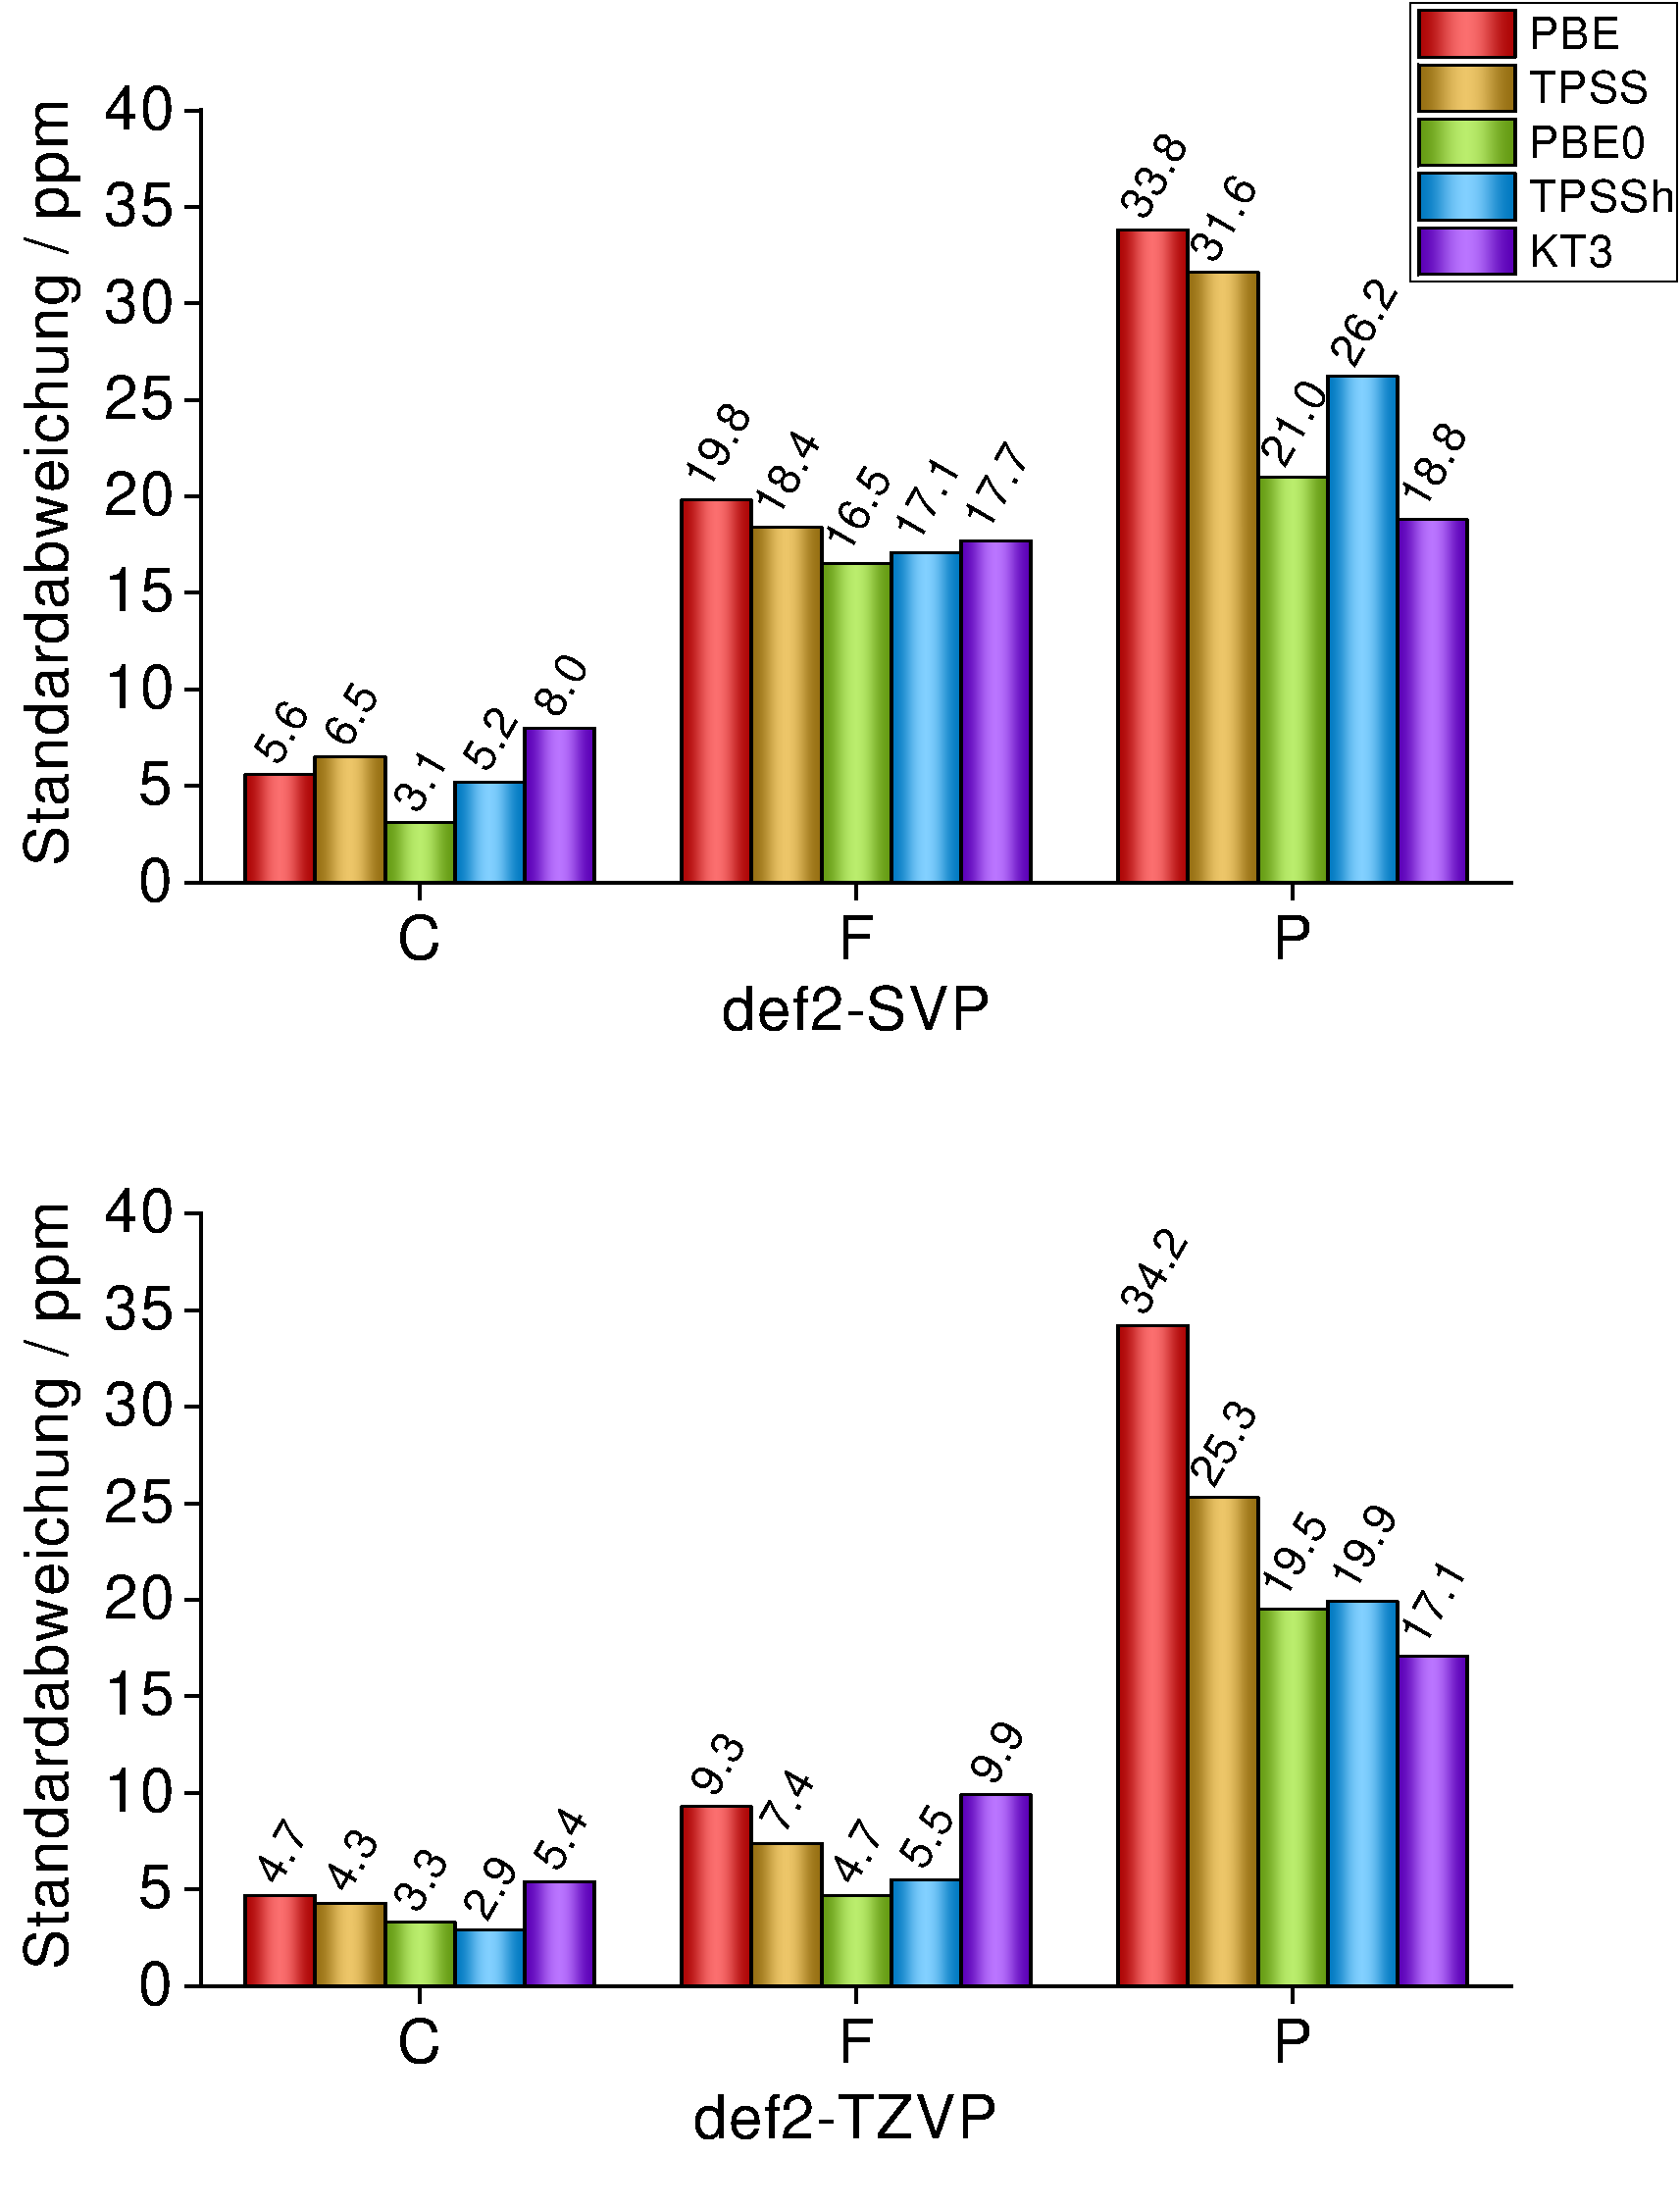
\includegraphics[width=0.72\textwidth]{cfpstd}
	\captionsetup{figurewithin = chapter}
	\captionsetup{font=small, labelfont=bf}\caption[Standardabweichungen für unterschiedliche Funktionale und Basissätze]{Standardabweichungen für C, F und P zwischen gemessenen und berechneten chemischen Verschiebungen in ppm für den Basissatz def2-SVP (oben) und den Basissatz def2-TZVP (unten). Die Verbindungen für die $^{13}$C-chemischen Verschiebungen wurden aus dem Testsatz von Referenz \cite{gauss1993effects} entnommen.} 
\label{abb:cfpshifts}
\end{figure}

\FloatBarrier
Neben den gerade beschriebenen allgemeinen Fehlern, die durch die \ac{dft} gemacht werden, wurden außerdem die zusätzlichen Fehler der in dieser Arbeit implementierten \ac{ri}- und \ac{marij}-Methoden untersucht. Für das \ac{ri}-Verfahren wurden erneut die weiter oben definierten Testsätze für die $^{13}$C-, $^{19}$F- und $^{31}$P-chemischen Verschiebung verwendet und mit den Werten ohne Verwendung der \ac{ri}-Näherung verglichen. Alle Rechnungen wurden unter Verwendung des TPSS-Funktionals und des Basissatzes def2-TZVP durchgeführt. Das \ac{ri}-Verfahren wurde dabei sowohl für die Optimierung der Strukturparameter als auch für die eigentliche Berechnung der chemischen Abschirmungskonstanten angewendet. Im Einzelnen sind die berechneten chemischen Verschiebungen in Tabelle \ref{tab:rierror} aufgelistet. Die Standardabweichung der Differenzen zu den Nicht-\ac{ri}-Rechnungen betragen \unit[0.04]{ppm} für $^{13}$C-chemische Verschiebungen, \unit[0.20]{ppm} für $^{19}$F-chemische Verschiebungen und \unit[0.41]{ppm} für $^{31}$P-chemische Verschiebungen und liegen damit etwa zwei bis drei Größenordnungen unterhalb des Fehlers der \ac{dft}-Rechnung an sich. Für die zusätzliche Beschleunigung durch das \ac{marij}-Verfahren sind die bisher betrachteten Moleküle zu klein, da nur wenige Integrale in den Fernfeld-Bereich fallen und damit durch die Multipolnäherung beschrieben werden würden. Aus diesem Grund wurden mithilfe des SWEET-Programms\supercite{bohne1999sweet} vier Einheiten der $\alpha$-\textsc{d}-Glucose erzeugt. Die kartesischen Koordinaten sowie die entsprechenden chemischen Abschirmungskonstanten sind in Tabelle \ref{tab:marijerror} aufgelistet. Beim Vergleich zischen \ac{ri} und \ac{marij} liegen die statistischen Größen \ac{maa}/\ac{sa}/\ac{maxa} für die $^{13}$C-Abschirmungskonstanten bei \unit[0.004/0.008/0.031]{ppm}, für die $^{1}$H-Abschirmungskonstanten dahingegen nur bei \unit[0.0003/0.0007/0.0038]{ppm}. Die zusätzlichen Fehler, die durch die Multipolnäherung eingeführt werden, sind damit vollkommen vernachlässigbar. Die entsprechenden Größen für den Vergleich zwischen der \ac{ri}- und Nicht-\ac{ri}-Rechnung betragen \unit[0.07/0.26/1.11]{ppm} für $^{13}$C und \unit[0.014/0.019/0.053]{ppm} für $^{1}$H. Auf einem einzelnen Intel\textsuperscript{\textregistered} Xeon\textsuperscript{\textregistered} Prozessor des Typs E5-2687W v2, 3.4 GHz betragen die Rechenzeiten für den Coulombteil \unit[4099]{s} ohne Näherung, \unit[220]{s} mit der \ac{ri}-Näherung und \unit[117]{s} mit der \ac{marij}-Näherung. Die Gesamtrechenzeit für die chemischen Abschirmungskonstanten betragen \unit[4610]{s}, \unit[741]{s} und \unit[633]{s}. Unter Verwendung der \ac{marij}-Methode entspricht dies im vorliegenden Fall einer Beschleunigung um einen Faktor 35 für den Coulombteil bzw. 7 für die gesamte Rechnung ohne einen signifikanten Verlust an Genauigkeit. 

Als weiteres Beispiel wurden die chemischen Abschirmungskonstanten mit dem PBE-Funktional und der Basis def2-SV(P) für ein \aclu*{rns-}\mbox{(\acs{rns}-)}\acused{rns}Segment (2kyd\supercite{2kydstructure}: [C$_{304}$H$_{346}$O$_{220}$N$_{118}$P$_{30}$]$^{30-}$, 10220 Basisfunktionen) berechnet. Die kartesischen Koordinaten wurden der Proteindatenbank entnommen und das System ist in Abbildung \ref{abb:2kyd} gezeigt. Aufgrund der großen negativen Ladung ist die Berechnung nur mithilfe des \ac{cosmo} möglich. Die Rechenzeiten für den Coulombteil betragen \unit[36.2]{h} ohne Näherung, \unit[3.4]{h} mit der \ac{ri}-Näherung und \unit[0.3]{h} mit der \ac{marij}-Näherung. Dies entspricht einer Beschleunigung der Berechnung des Coulombteils um einen Faktor größer als 100. Die Gesamtrechenzeiten betragen \unit[43.2]{h}, \unit[10.7]{h} und \unit[7.6]{h} Stunden, was einem Faktor von etwa 6 auf die Gesamtrechenzeit ergibt. Ein Großteil der verbleibenden Rechenzeit wird für die Berechnung der zahlreichen \ac{cosmo}-Integrale benötigt, wodurch die Beschleunigung der Gesamtrechenzeit hier etwas moderater ausfällt. Jedoch wurde insgesamt, wie auch in den anderen Beispielen, die Zeit für die Berechnung der Wellenfunktion unterboten. Mit der \ac{marij}-Näherung liegt diese bei \unit[9.9]{h}.

\begin{figure}[ht!]
	\centering
	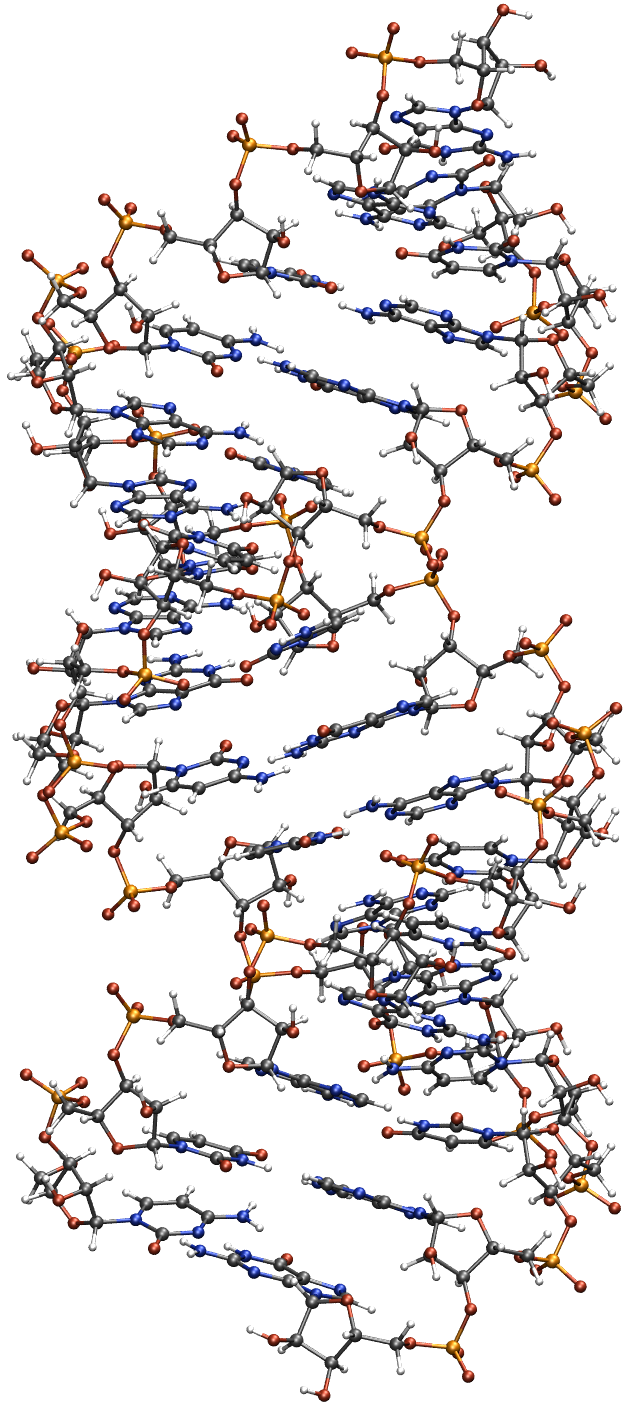
\includegraphics[width=0.6\textwidth]{2kyd}
	\captionsetup{figurewithin = chapter}
	\captionsetup{font=small, labelfont=bf}\caption[{Abbildung eines \ac{rns}-Segmentes}]{Abbildung des \ac{rns}-Segmentes 2kyd\supercite{2kydstructure}: [C$_{304}$H$_{346}$O$_{220}$N$_{118}$P$_{30}$]$^{30-}$ (Kohlenstoff=grau, Wasserstoff=weiß, Sauerstoff=rot, Stickstoff=blau und Phosphor=orange).}
\label{abb:2kyd}
\end{figure}

\bigskip
Neben der Genauigkeit wurde des Weiteren auch die Effizienz der neu implementierten Methoden untersucht. Zunächst wurde dafür das Skalierungsverhalten mit der Molekülgröße für eine gegebene (kleine) Basis betrachtet. Analog zu bisher bestehenden Implementierungen\supercite{beer2011nuclei,kumar2016nuclei} wurden dafür $n$ verknüpfte $\alpha$-\textsc{d}-Glucose-Einheiten mit $n=1,2,4,8,16,32,48,64,128$ betrachtet. Die Strukturen wurden erneut mit dem SWEET-Programm erzeugt. Für die Berechnungen wurde dasselbe Funktional B3LYP\supercite{becke1993density,lee1988development,stephens1994ab} sowie dieselbe Basis/Auxiliarbasis 6-31G$^*$\supercite{hariharan1973influence}/def2-SV(P)\supercite{eichkorn1995auxiliary} verwendet. Zusätzlich wurden noch Berechnungen für die Funktionale PBE, TPSS und TPSSh durchgeführt. Bei allen Berechnungen wurde die Beschleunigung durch die \ac{marij}-Näherung ausgenutzt. Die einzelnen Rechenzeiten auf einem einzelnen Intel\textsuperscript{\textregistered} Xeon\textsuperscript{\textregistered} Prozessor des Typs E5-2687W v2, 3.4 GHz sind in Tabelle \ref{tab:sizeskaling} aufgelistet. 

\begin{table}[ht!]
\centering
\small
\captionsetup{tablewithin = chapter}
\captionsetup{font=small, labelfont=bf}
\captionabove[Rechenzeiten der Abschirmungskonstanten für $n$ verknüpfte $\alpha$-D-Glucose Einheiten]{Rechenzeiten der Abschirmungskonstanten für $n$ verknüpfte $\alpha$-\textsc{d}-Glucose-Einheiten mit unterschiedlichen Funktionalen und dem 6-31G$^*$/def2-SV(P) Basis-/Auxiliarbasissatz. Die Berechnungen wurden auf einem einzelnen Intel\textsuperscript{\textregistered} Xeon\textsuperscript{\textregistered} Prozessor E5-2687W v2, 3.4 GHz durchgeführt. Die Spalten \glqq abs\grqq{} beinhalten absolute Rechenzeiten in Stunden. Für die Hybridfunktionale ist in Klammern die Anzahl der \ac{cphf}-Iterationen angegeben. Die Spalten \glqq rel\grqq{} geben das Verhältnis der Rechenzeit zur vorausgehenden \ac{scf}-Rechnung an. Diese wurden jeweils beginnend mit Hückelorbitalen durchgeführt und konvergierten in 10--17 Iterationen.}
%\resizebox{\textwidth}{!}{%
    \begin{tabular}{S[table-format = 3.0]S[table-format = 2.3]S[table-format = 1.2]S[table-format = 2.3]S[table-format = 1.2]S[table-format = 2.3]@{\hspace{2pt}}rS[table-format = 1.2]S[table-format = 2.3]@{\hspace{5pt}}rS[table-format = 1.2]}
    \hline \hline
          & \multicolumn{2}{c}{PBE} & \multicolumn{2}{c}{TPSS} & \multicolumn{3}{c}{B3LYP} & \multicolumn{3}{c}{TPSSh} \\
    \hline
    $n$     & \text{abs}   & \text{rel}   & \text{abs}   & \text{rel}   & \multicolumn{2}{c}{\text{abs}}   & \text{rel}   & \multicolumn{2}{c}{\text{abs}}   & \text{rel} \\
    1     & 0.003 & 0.75  & 0.005 & 0.83  & 0.009 &(5) & 0.75  & 0.010 &(5) & 0.71 \\
    2     & 0.010 & 0.77  & 0.014 & 0.70  & 0.036 &(7) & 0.76  & 0.035 &(6) & 0.70 \\
    4     & 0.028 & 0.60  & 0.039 & 0.61  & 0.120 &(8) & 0.76  & 0.116 &(6) & 0.71 \\
    8     & 0.079 & 0.60  & 0.103 & 0.65  & 0.389 &(8) & 0.93  & 0.342 &(6) & 0.82 \\
    16    & 0.246 & 0.68  & 0.288 & 0.69  & 1.00 &(9) & 1.00  & 0.914 &(7) & 0.87 \\
    32    & 0.887 & 0.67  & 0.964 & 0.59  & 2.91 &(10) & 1.02  & 2.64 &(7) & 0.92 \\
    48    & 2.00  & 0.55  & 2.15  & 0.49  & 5.75 &(10) & 0.93  & 5.42 &(8) & 0.83 \\
    64    & 3.59  & 0.45  & 3.76  & 0.41  & 10.02 &(10) & 0.83  & 9.48 &(8) & 0.79 \\
    128   & 17.31 & 0.35  & 18.10 & 0.31  & 51.01 &(11) & 0.77  & 42.99 &(8) & 0.66 \\
    \end{tabular}%}%
  \label{tab:sizeskaling}%
\end{table}%

\FloatBarrier

Für das größte System mit $n=128$ (2691 Atome, 23699 Basisfunktionen) kann die Berechnung der chemischen Abschirmungskonstanten auf einer CPU innerhalb eines Tages bzw. zweier Tage bei der Verwendung von reinen bzw. Hybridfunktionalen durchgeführt werden. Für Letztere benötigten die vorausgehenden Berechnungen der Wellenfunktion, welche innerhalb von 10 bis 17 Iterationen konvergierten, etwa genau so viel Zeit wie die eigentlichen Berechnungen der chemischen Abschirmungskonstanten. Tendenziell verbessert sich dieses Verhältnis zugunsten der \ac{nmr}-Rechnung bei großen Systemen. Bei reinen Dichtefunktionalen ohne Hartree-Fock-Austausch ist die Berechnung der Abschirmungskonstanten deutlich schneller als die vorausgehende \ac{scf}-Rechnung. Insgesamt wird für reine Dichteunktionale ein Skalierungsverhalten von $\mathcal{O}(n^{1.8})$ und für Hybridfunktionale ein Skalierungsverhalten von $\mathcal{O}(n^{1.7})$ mit der Systemgröße erhalten. Für die kleineren Systeme bis $n=16$ ist dieses Skalierungsverhalten noch besser. Bei den größeren Systemen beginnen dann $n^3$-Schritte dominant zu werden, was zu einem Skalierungsverhalten von mehr als $\mathcal{O}(n^{2})$ mit der Systemgröße führt. Im Wesentlichen sind das die Diagonalisierung bei der \ac{scf}-Rechnung sowie die Berechnung der Ableitungen nach den Komponenten der Kernmomente für jedes Atom. Die Berechnung für $n=48$ mit dem B3LYP-Funktional, was das größte berechnete System in der bisher aktuellsten Implementierung aus Referenz \cite{kumar2016nuclei} darstellt, benötigt dort \unit[19.8]{h} auf 16 CPUs. Im Vergleich dazu liegt die Rechenzeit mit der in dieser Arbeit vorliegenden Implementierung, wohlgemerkt auf einer CPU, bei weniger als einem Drittel (\unit[5.75]{h}). 

\bigskip
Abgesehen von der bisherigen Betrachtung des Skalierungsverhaltens beim Vergrößern der Systemgröße, wurde auch der Einfluss einer größeren Basis bei gleicher Systemgröße untersucht. Für das System mit $n=16$ wurde daher die Basis def2-TZVP verwendet, welche etwa 2.5 mal so groß wie die bisher betrachtete Basis 6-31G$^*$ ist. Bei der Verwendung des TPSS-Funktionals führt dies zu einer Verlängerung der Rechenzeit für die Abschirmungskonstanten um einen Faktor von ca. 4.6 und damit zu einem Skalierungsverhalten von $\mathcal{O}(n^{1.7})$ ($\frac{\log(4.6)}{\log(2.5)}$). Die Berechnung mit dem Hybridfunktional TPSSh führt zu einer Verlängerung um einen Faktor von ca. 19 und damit zu einem deutlich weniger guten Skalierungsverhalten von etwa $\mathcal{O}(n^{3.2})$. Dies kann dadurch begründet werden, dass durch die größere Basis im Wesentlichen Funktionen mit größerer $l$-Quantenzahl hinzugefügt werden. Deren Beiträge können zum großen Teil nicht bei der Integralabschätzung vernachlässigt werden, wodurch das eigentliche Skalierungsverhalten nicht weit vom formalen Skalierungsverhalten mit $\mathcal{O}(n^{4})$ entfernt liegt. Abhilfe lässt sich möglicherweise durch die Implementierung der \ac{ri}-Methode für den Austausch, \ac{ri}-\textit{K}\supercite{weigend2002fully}, oder durch seminumerische Berechnung\supercite{neese2009efficient,plessow2012seminumerical} des Letzteren schaffen. Die parallele Ausführung des Programms auf 4 CPUs führt für das System mit $n=32$ und der Basis 6-31G$^*$ zu einer Beschleunigung der Berechnung um einen Faktor von ca. 3.1, für das System mit $n=16$ und der Basis def2-TZVP zu einer Beschleunigung um einen Faktor von ca. 3.6. Dies trifft sowohl auf die Verwendung reiner \ac{dft}-Funktionale als auch auf Hybridfunktionale zu.
